\section{Tests préliminaires \label{test_vision}}
Le but des tests préliminaires est de vérifier que les analyses effectuées dans la phase de recherche sont applicables et nous retournent
des résultats exploitables. Ils permettent également de se rendre compte si le système imaginé lors de la sélection du matériel est en accord avec
ce qui est réalisable.
\subsection{Matériel}
Au moment des tests, les élements suivants étaient à ma disposition :
\begin{itemize}
    \item 1x Rapsberry Pi 4b - 4Go de RAM.
    \item 1x Pi caméra module 3 NoIR Wide.
    \item 20x leds IR 830nm.
    \item 20x leds IR 850nm.
    \item 20x leds IR 880nm.
    \item 1x morceau de route.
    \item 1l. Huile de moteur neuf - 15W-40.
\end{itemize}

\subsection{Eclairage}
L'éclairage utilisé dans le cadre des tests préliminaires consiste en deux rails de leds IR montées en ligne sur deux veroboards.
Le montage a été effectué selon le schéma suivant:
\begin{figure}[H]
    \centering
    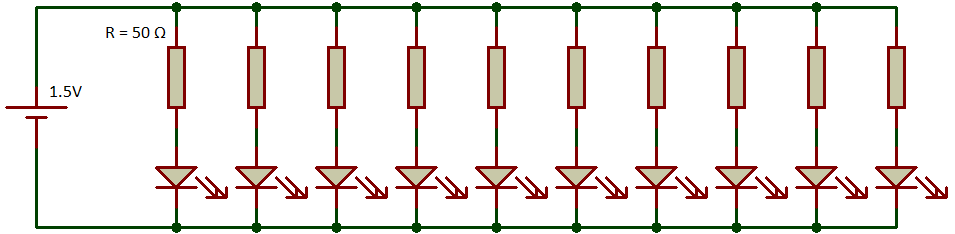
\includegraphics[width=13cm]{assets/figures/schema_leds1.png}
    \caption{Eclairage de test - Schéma électrique de la rangée de led - Schéma modifié de: https://www.sonelec-musique.com/electronique_realisations_alim_led.html}
\end{figure}
Les veroboards sont pratiques à manipuler, il est possible se les tenir avec des étaux afin de faire varier les positions durant les tests. Une fois monté,
le résultat est le suivant:
\begin{figure}[H]
    \centering
    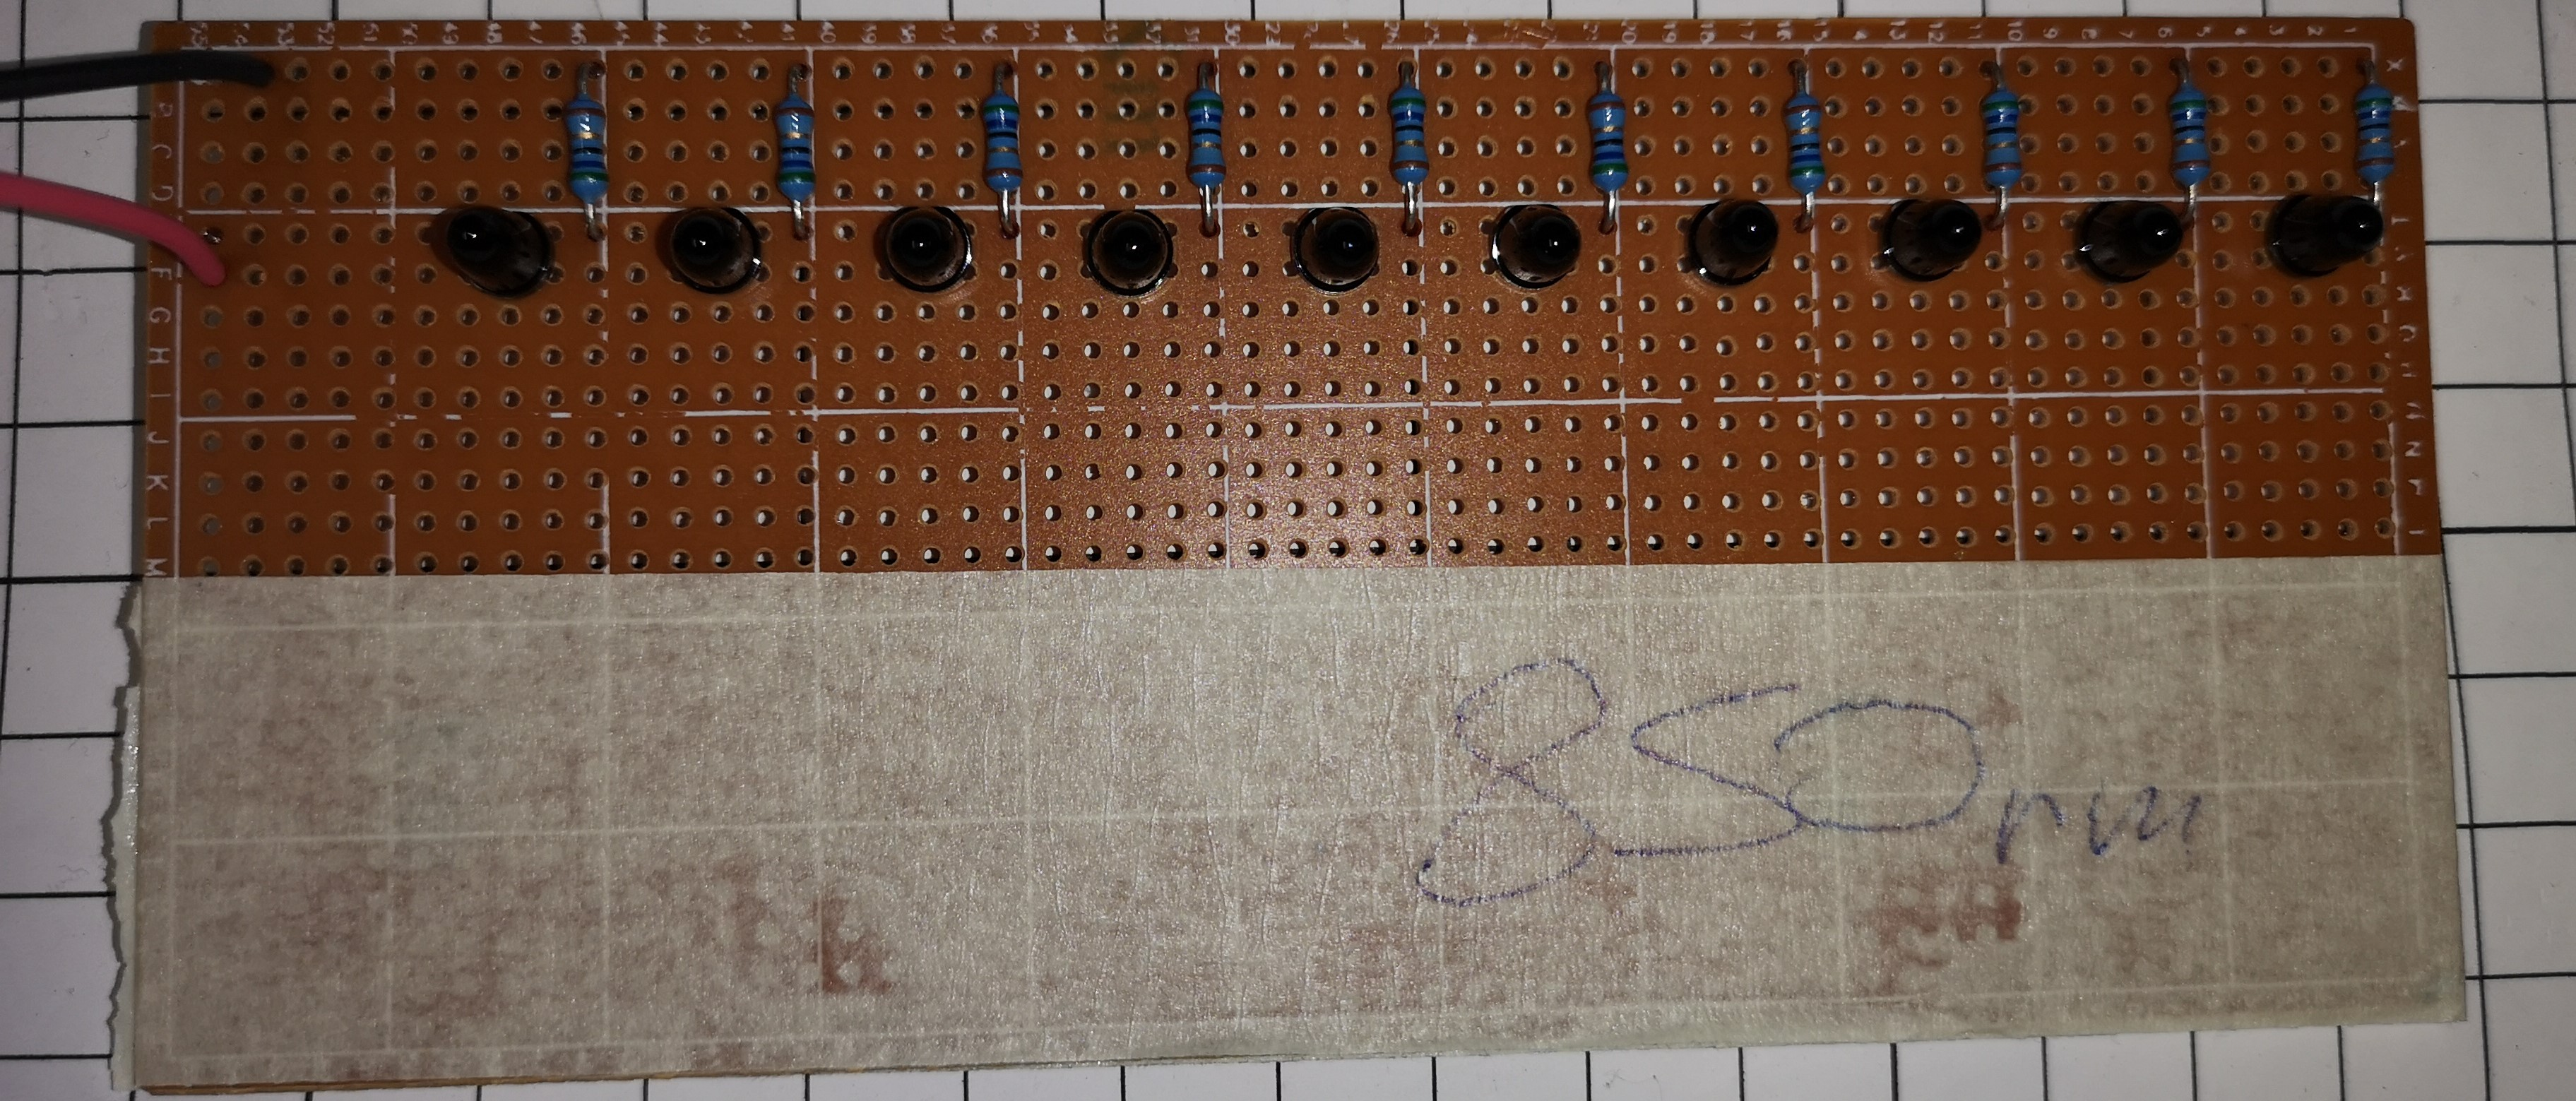
\includegraphics[width=13cm]{assets/figures/rail_led1.jpg}
    \caption{Eclairage de test - Rail de leds 1}
\end{figure}

\begin{figure}[H]
    \centering
    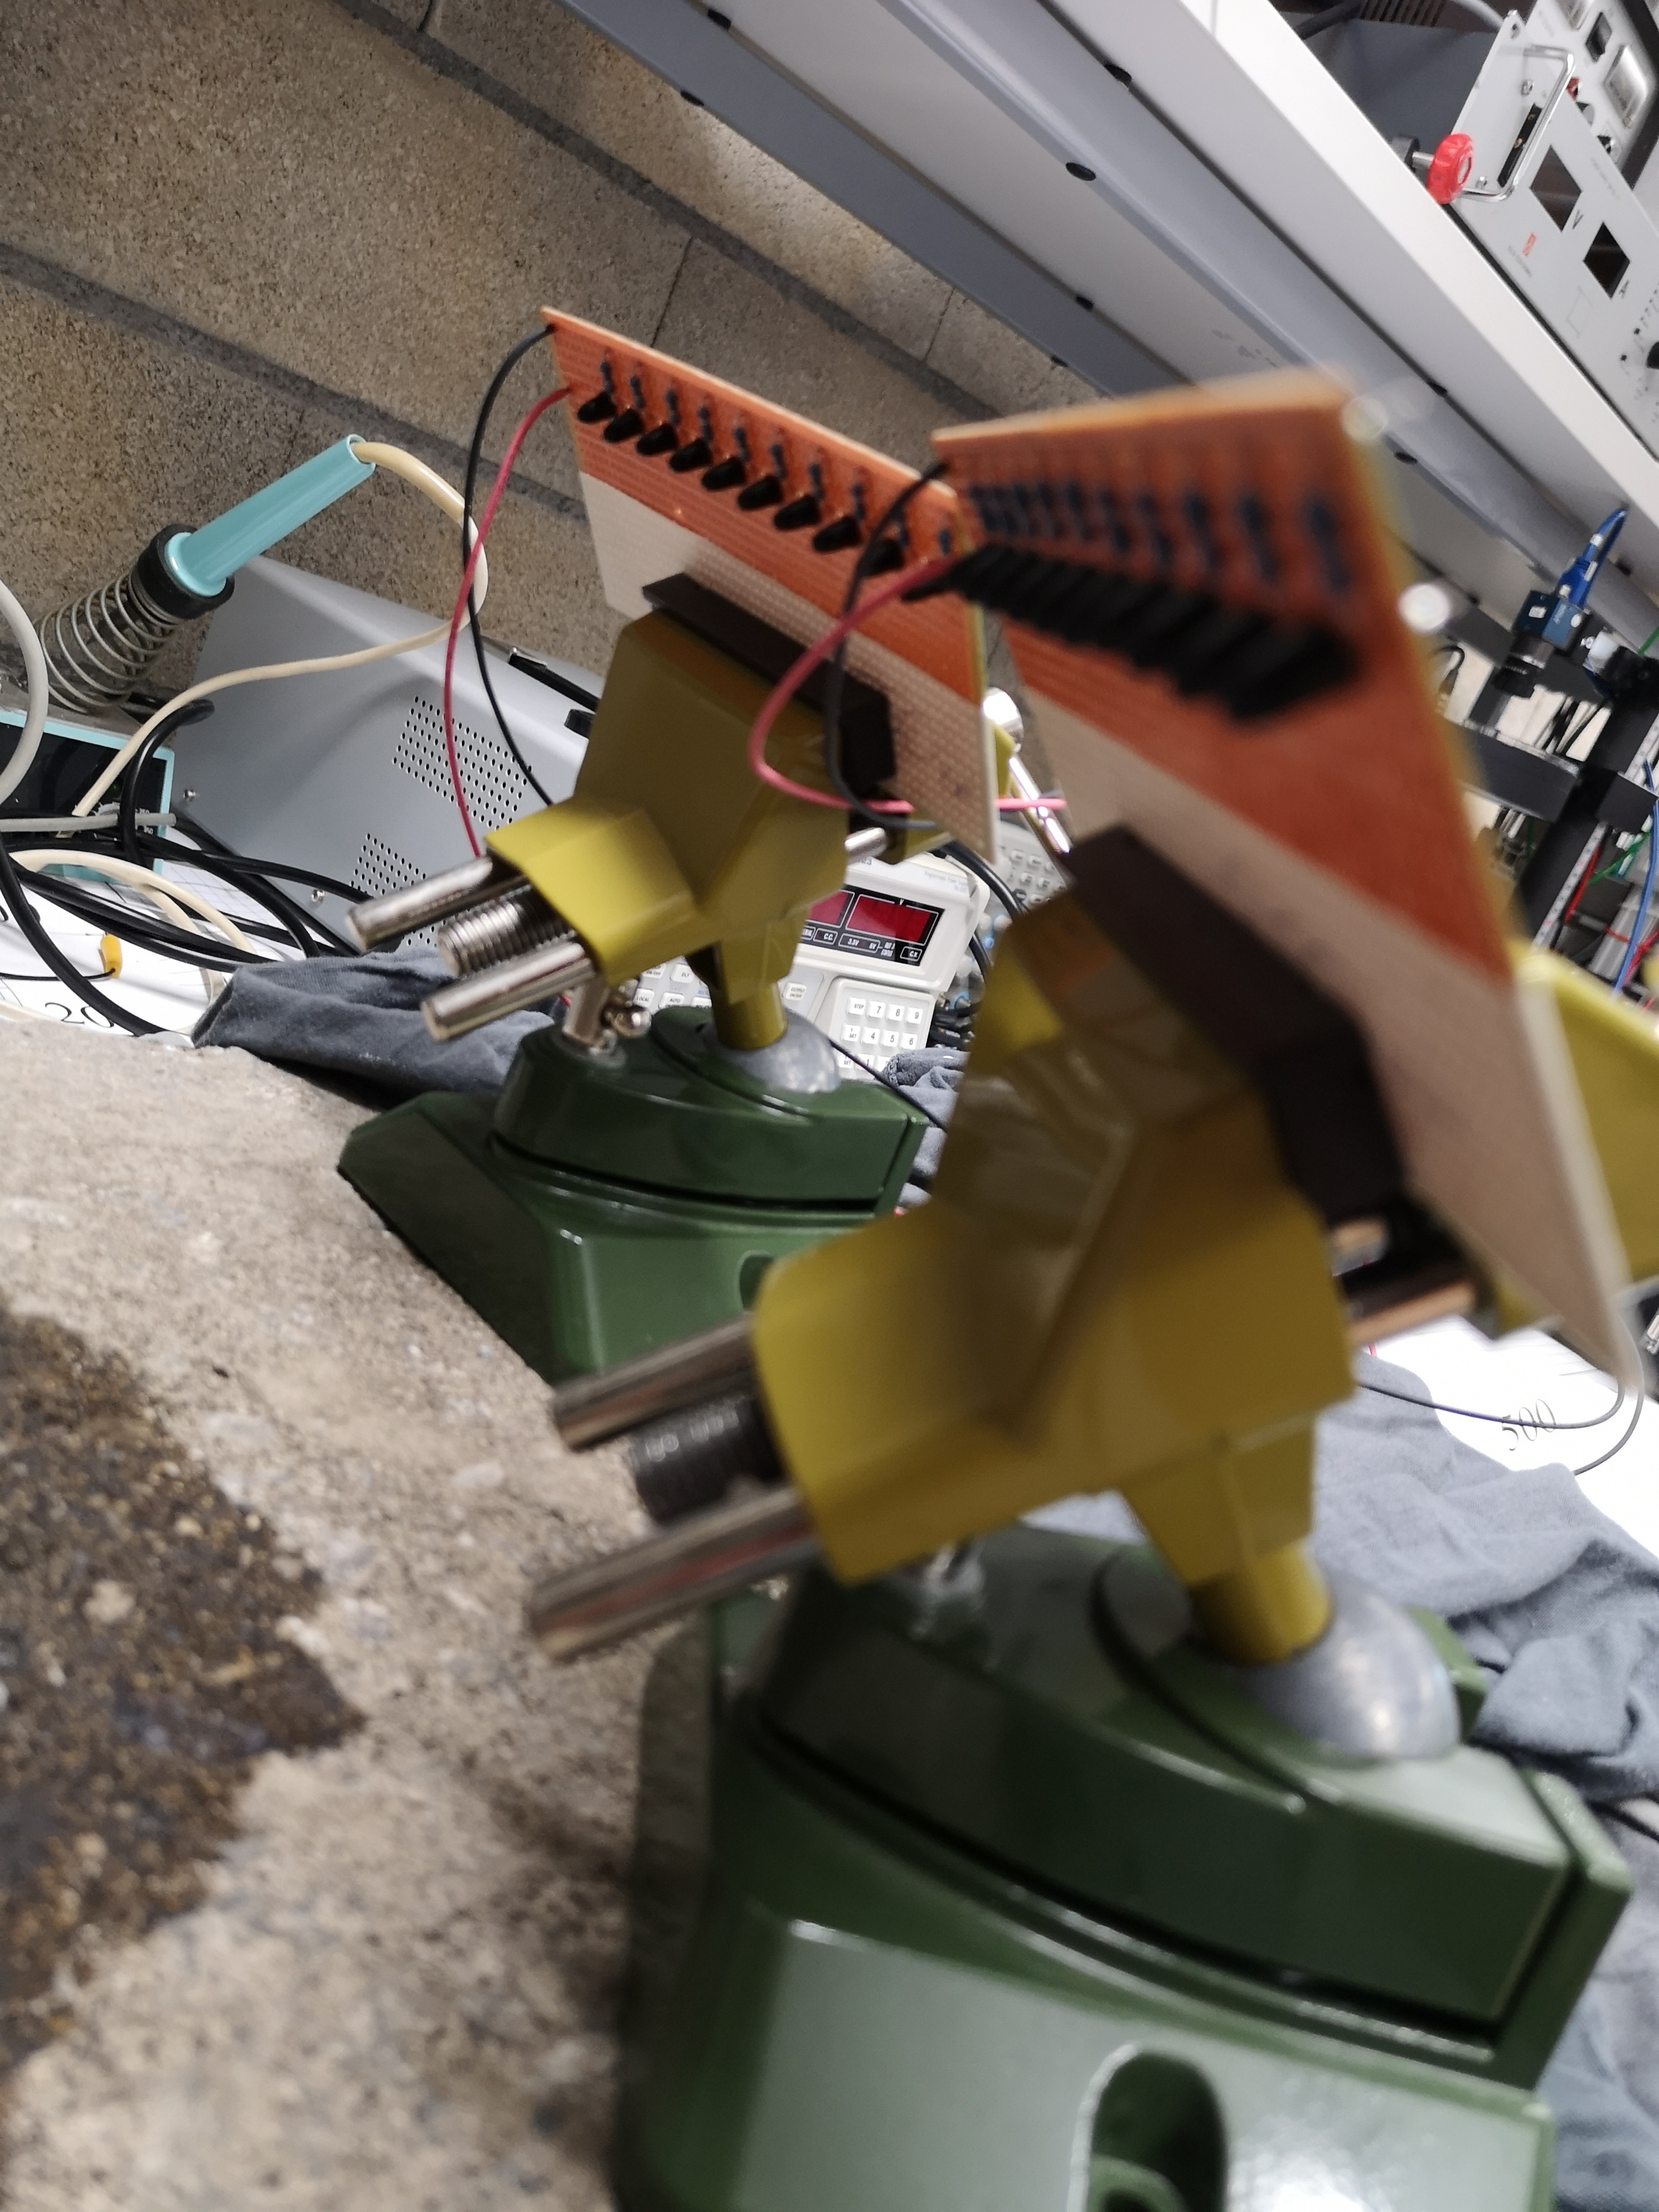
\includegraphics[width=8cm]{assets/figures/rail_led2.jpg}
    \caption{Eclairage de test - Rail de leds 2}
\end{figure}
\subsection{Capture}
La capture d'acquisition des images de tests préliminaires se fait via la caméra sélectionnée durant la phase de décision, un Rpi4 ainsi
qu'un petit script configurant la caméra et enregistrant l'image.
\subsection{Images}
Vu depuis la caméra, nous avons la scène suivante:

\begin{figure}[H]
    \centering
    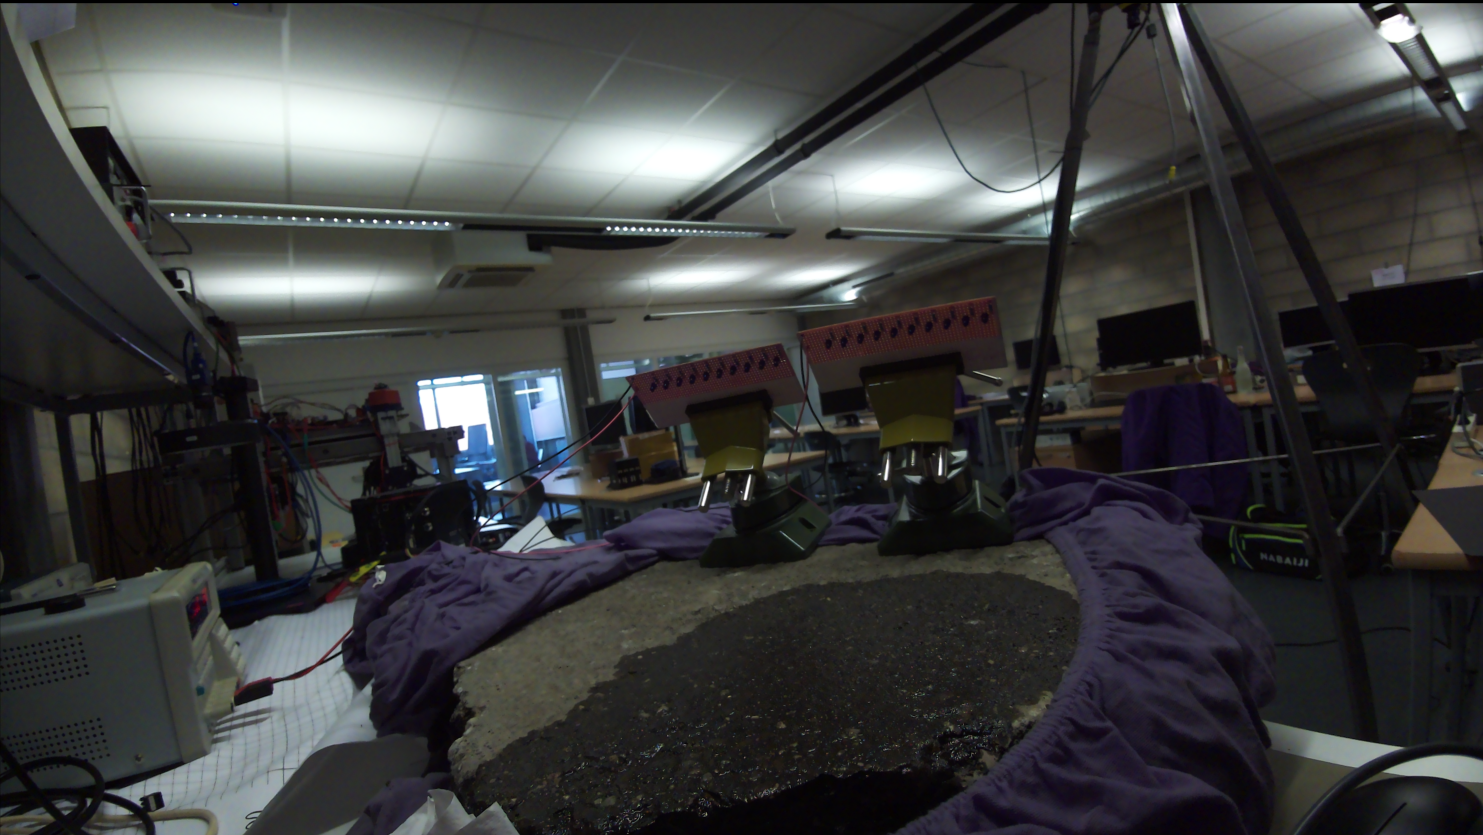
\includegraphics[width=13cm]{assets/figures/camera_vue_couleur1.png}
    \caption{Capture de test - Vue de la scène en couleur}
\end{figure}

Au moment d'effectuer les tests de sensibilités aux IR, tout le matériel n'était pas encore arrivé, notement le filtre de l'objectif ne
laissant passer que les infrarouges. J'ai donc effectué les captures qui vont suivre dans les conditions suivantes:
\begin{itemize}
    \item Lumières éteintes dans la pièce.
    \item Deux lignes de 10 leds IR éclairant en direction de la tâche d'huile de moteur.
    \item Protection contre les lumières parasites du couloir (carton).
    \item Auto-focus sur le centre de l'image
    \item Temps d'exposition: 5000[ns]. (déterminé expérimentalement avec plusieurs captures)
\end{itemize}
Avec ce setup, j'ai effectué plusieurs captures en faisant varier la position de l'éclairage par rapport à la tâche d'huile et la caméra.
J'ai obtenu différents résultats, plus ou moins utilisables.


Ci-dessous, un exemple d'éclairage orienté "contre" la caméra selon la figure suivante:
\begin{figure}[H]
    \centering
    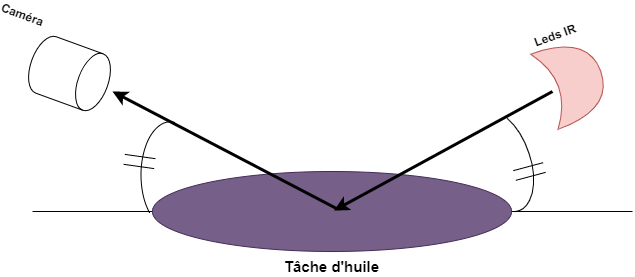
\includegraphics[width=13cm]{assets/figures/eclairage_contre_camera.png}
    \caption{Schéma de capture - Eclairage contre la camera \label{led_perp}}
\end{figure}


\begin{figure}[H]
    \centering
    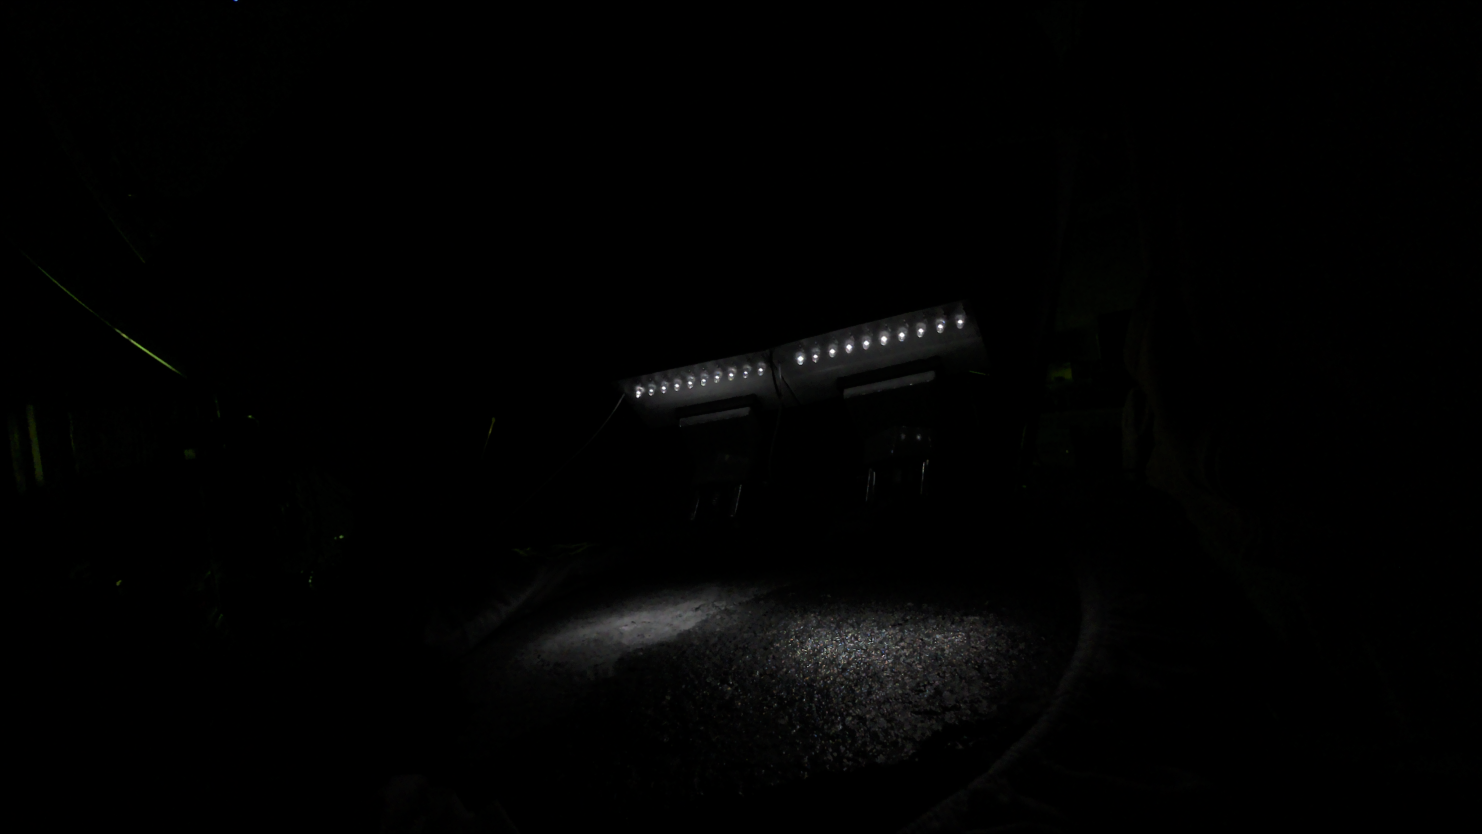
\includegraphics[width=13cm]{assets/figures/eclairage_face1.png}
    \caption{Capture de test - éclairage de face 1}
\end{figure}
\begin{figure}[H]
    \centering
    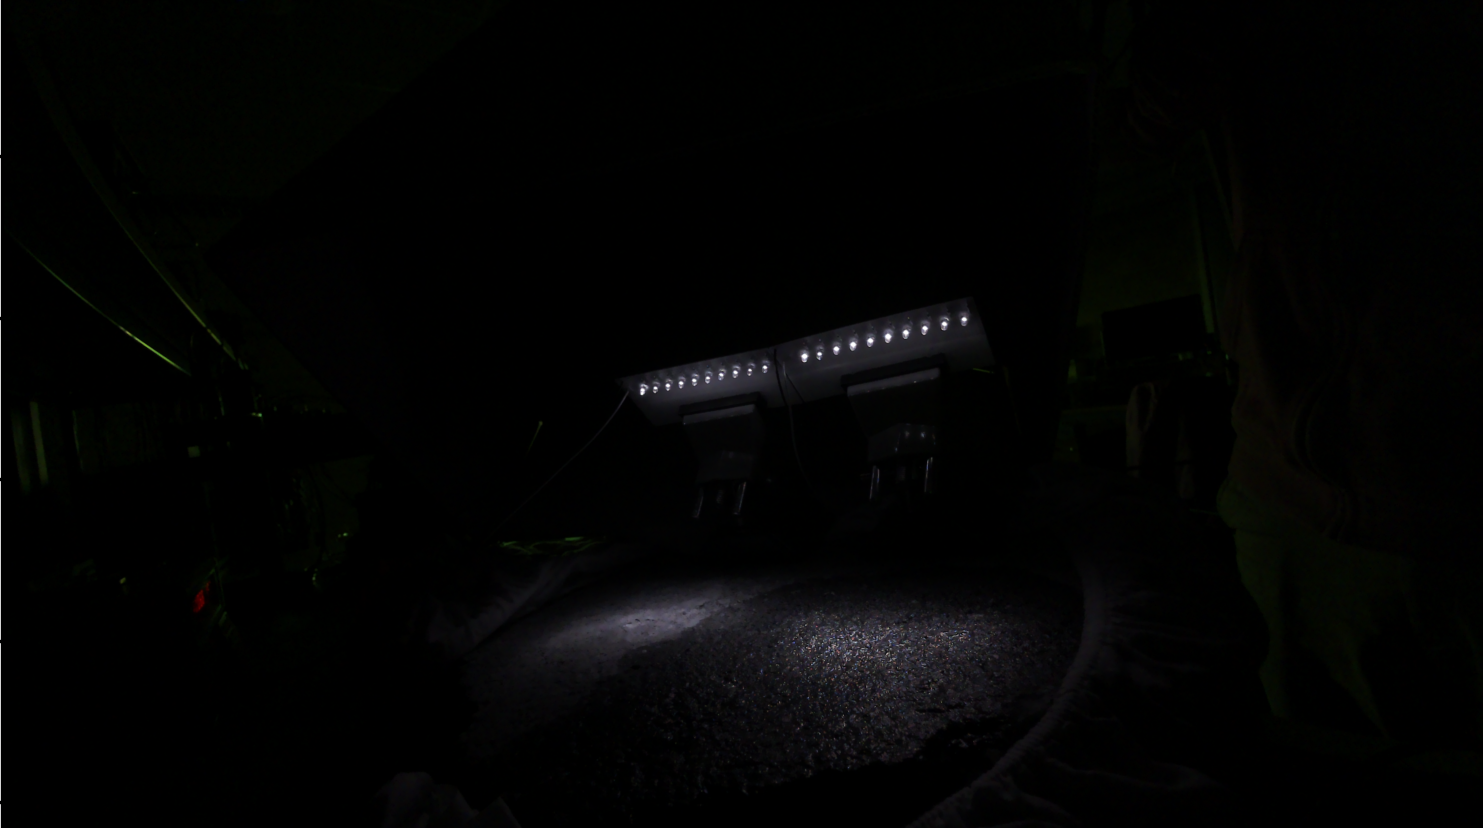
\includegraphics[width=13cm]{assets/figures/eclairage_face2.png}
    \caption{Capture de test - éclairage de face 2}
\end{figure}

On observe que la route et l'huile reflètent les leds IR, à l'oeil nu la différence est notable, mais l'analyse avec un soft peut s'avérer compliquée.\\
Ci-dessous, un exemple d'éclairage orienté perpendiculairement à la route selon la figure suivante:
\begin{figure}[H]
    \centering
    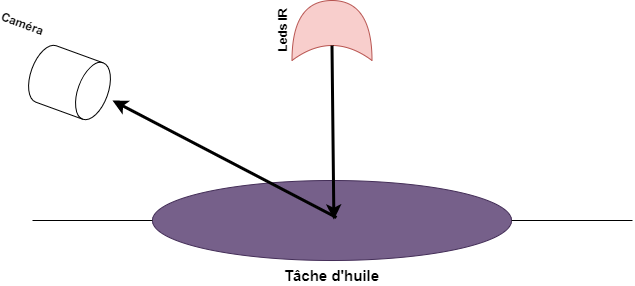
\includegraphics[width=13cm]{assets/figures/eclairage_perpendiculaire.png}
    \caption{Schéma de capture - Eclairage perpendiculaire à la route}
\end{figure}

\begin{figure}[H]
    \centering
    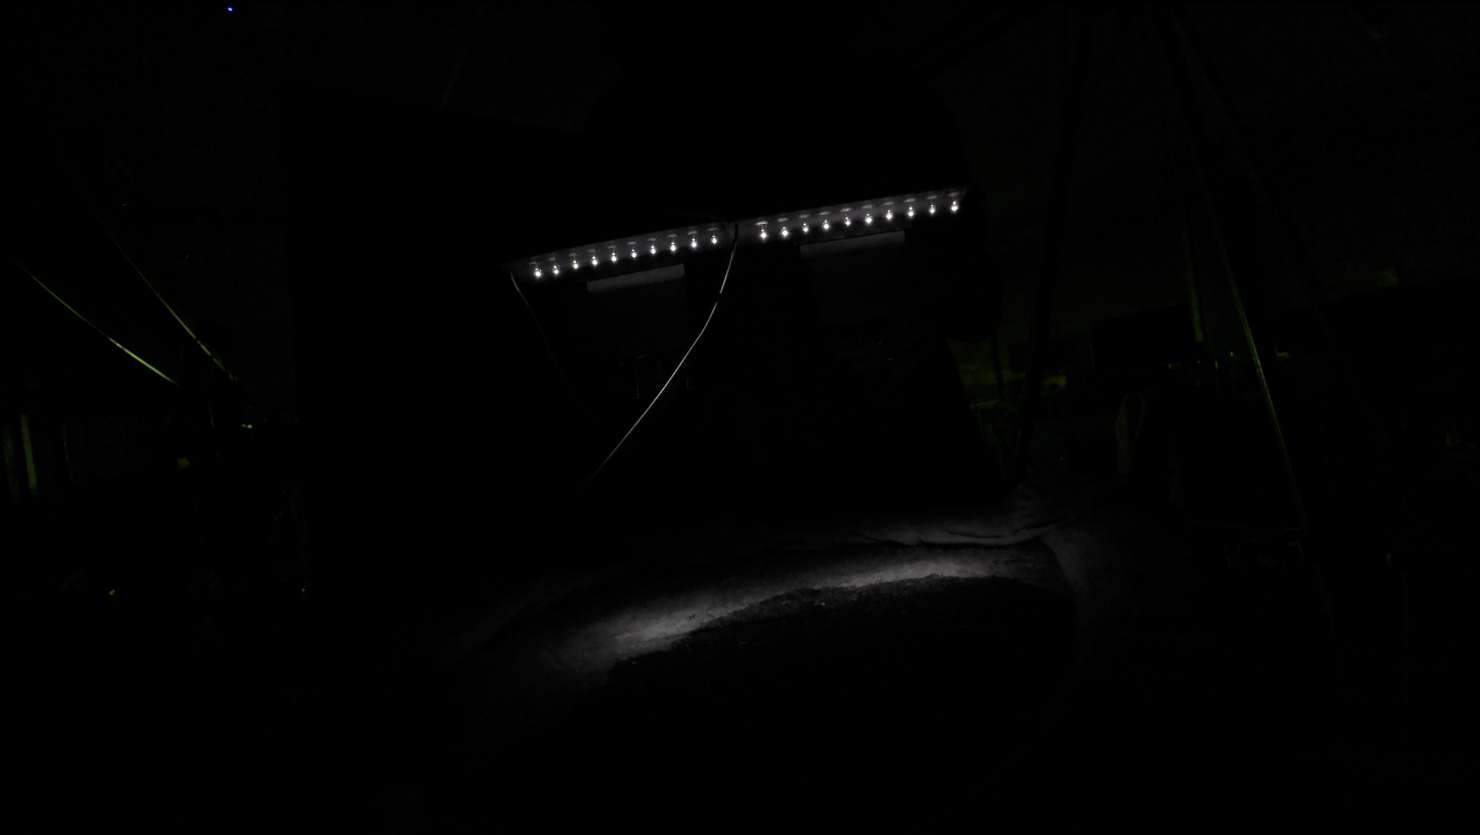
\includegraphics[width=13cm]{assets/figures/eclairage_perpendiculaire1.png}
    \caption{Capture de test - Eclairage perpendiculaire 1}
\end{figure}
\begin{figure}[H]
    \centering
    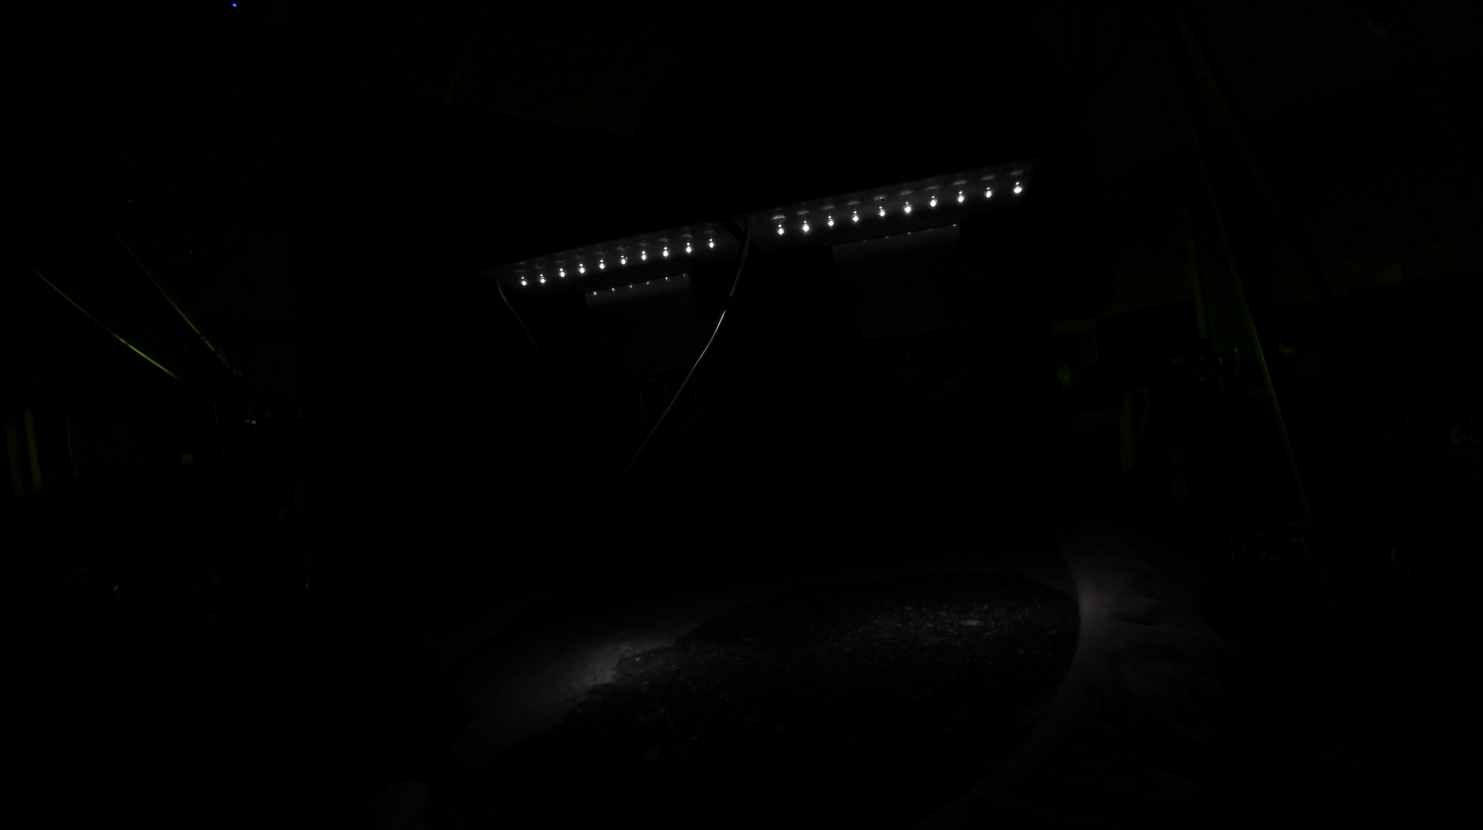
\includegraphics[width=13cm]{assets/figures/eclairage_perpendiculaire2.png}
    \caption{Capture de test - Eclairage perpendiculaire 2}
\end{figure}

\begin{figure}[H]
    \centering
    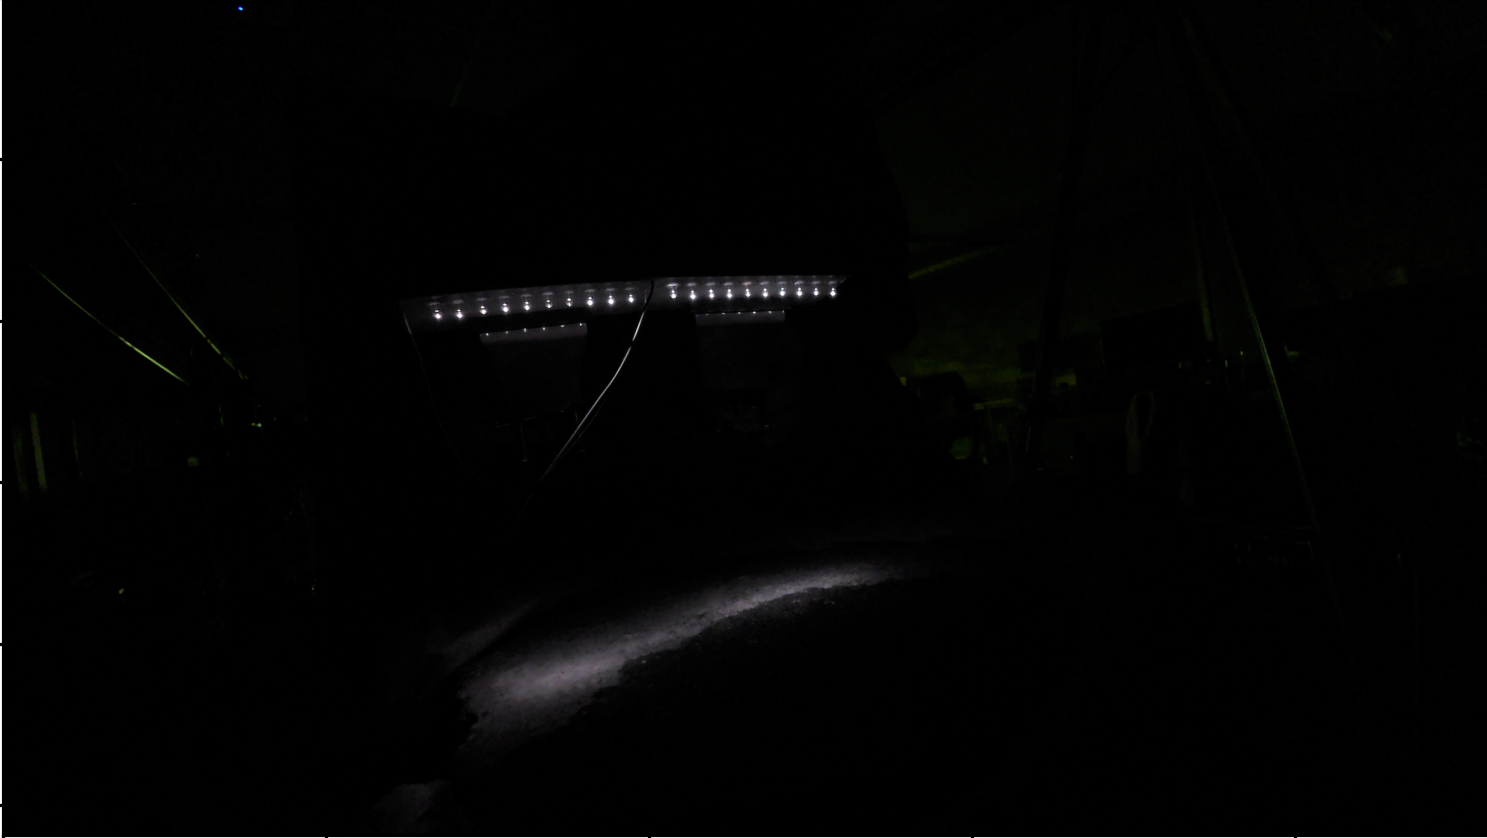
\includegraphics[width=13cm]{assets/figures/eclairage_perpendiculaire3.png}
    \caption{Capture de test - Eclairage perpendiculaire 3}
\end{figure}
On observe que la route diffuse, dans une moindre mesure, l'éclairage des leds IR, là ou l'huile semble absorber les rayonnements. On arrive
assez facilement à différencier le clair de la route et le foncé de l'huile. La mise en place d'un software de détection est envisageable avec
un éclairage basé sur ce schéma. A noter que les tests ont été effectués avec plusieurs gammes de leds (830nm, 850nm et 880nm), la différence
sur le retour image n'est pas très grandes, mais les leds 850nm permettent de mieux différencier la route de l'huile.
\newpage
J'ai également tenté la configuration suivante:
\begin{figure}[H]
    \centering
    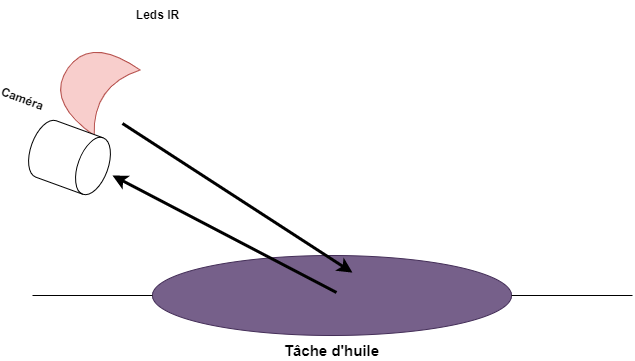
\includegraphics[width=13cm]{assets/figures/eclairage_dos.png}
    \caption{Schéma de capture - Eclairage de dos}
\end{figure}
Mais, étant trop sombre, les images obtenues n'étaient pas utilisables.
\subsection{Filtre du visible}
J'ai effectué quelques tests supplémentaires après la réception des filtres ne laissant passer que l'infrarouge. Pour rappel, le filtre
ne laisse passer que les ondes supérieures à 700nm, les rouges lointains seront encore visibles.

\begin{figure}[H]
    \centering
    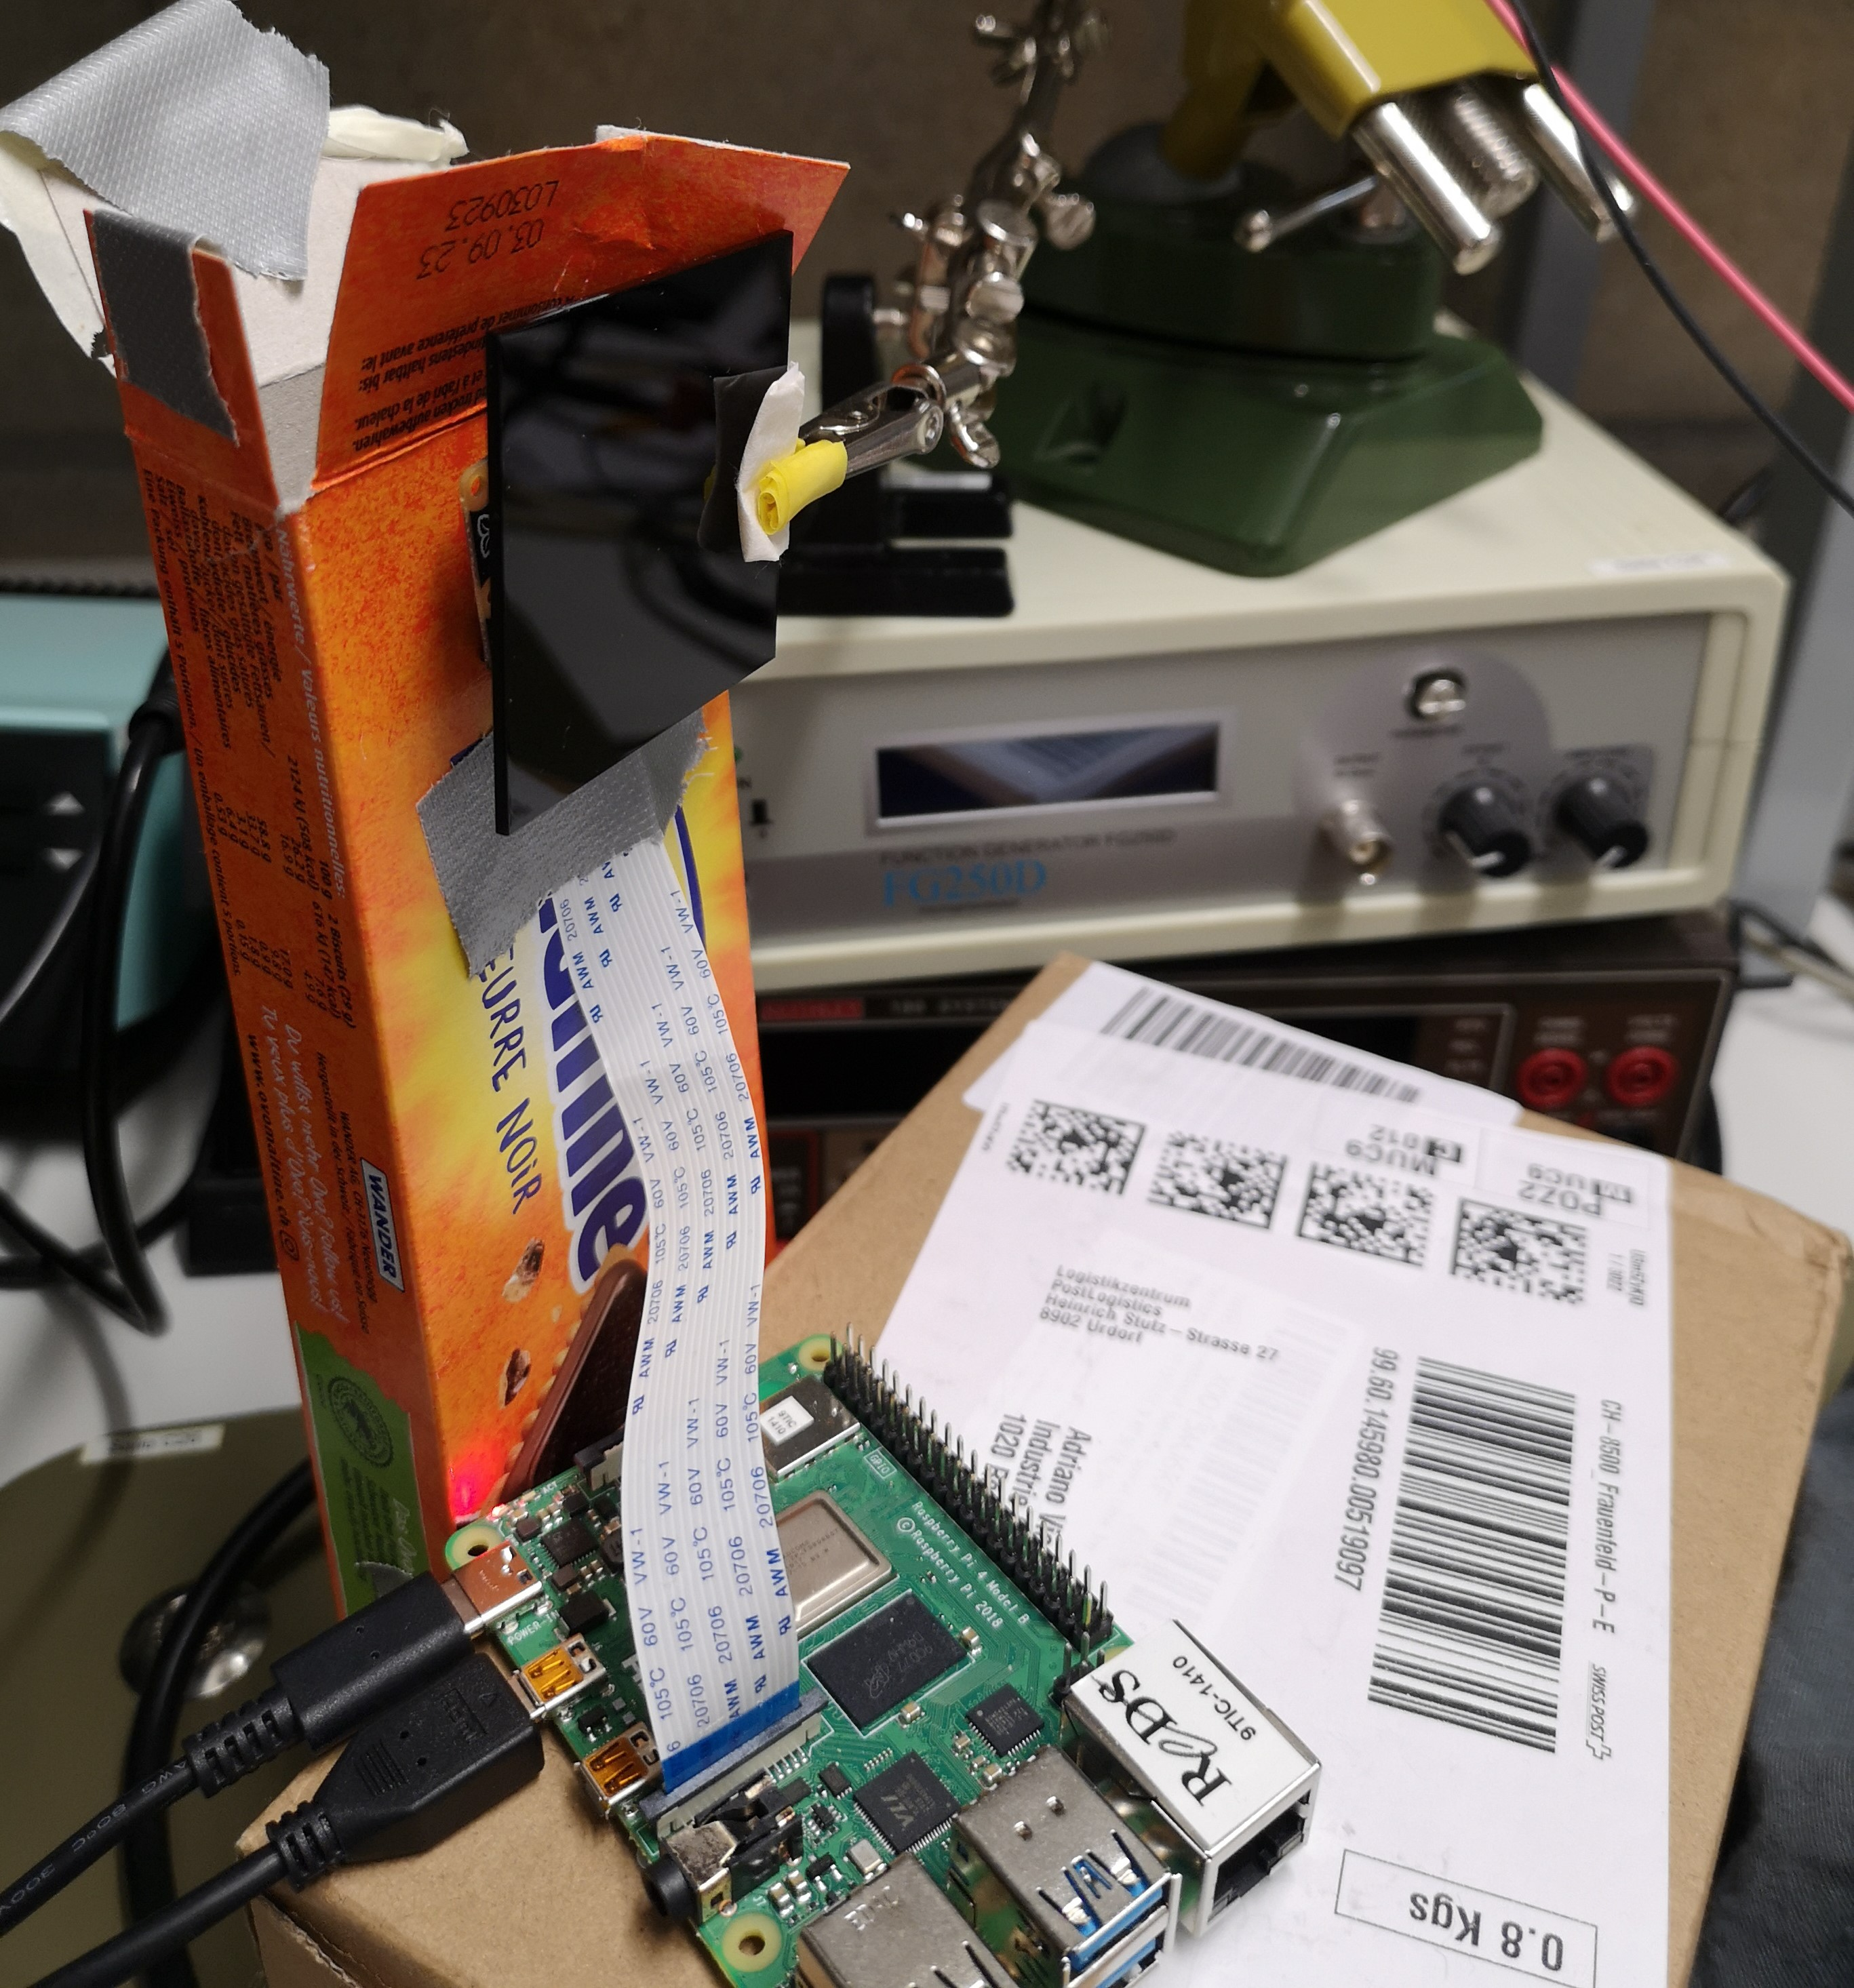
\includegraphics[height=13cm]{assets/figures/filtre.jpg}
    \caption{Capture avec filtre - Installation}
\end{figure}

Pour constater l'efficacité du filtre, j'ai effectué 3 captures.
\begin{itemize}
    \item Une image simple.
    \item Une image avec l'éclairage IR enclenché.
    \item Une image avec l'éclairage IR enclenché selon la figure \ref{led_perp}.
\end{itemize}
On notera également que le filtre perturbe l'autofocus du capteur, la position de la lentille a donc été définie en dur dans le code de test.
Les informations concernant ces réglages se trouvent au chapitre 5.2.3 de la documentation Picamera2 \cite{picamera2}.

\begin{figure}[H]
    \centering
    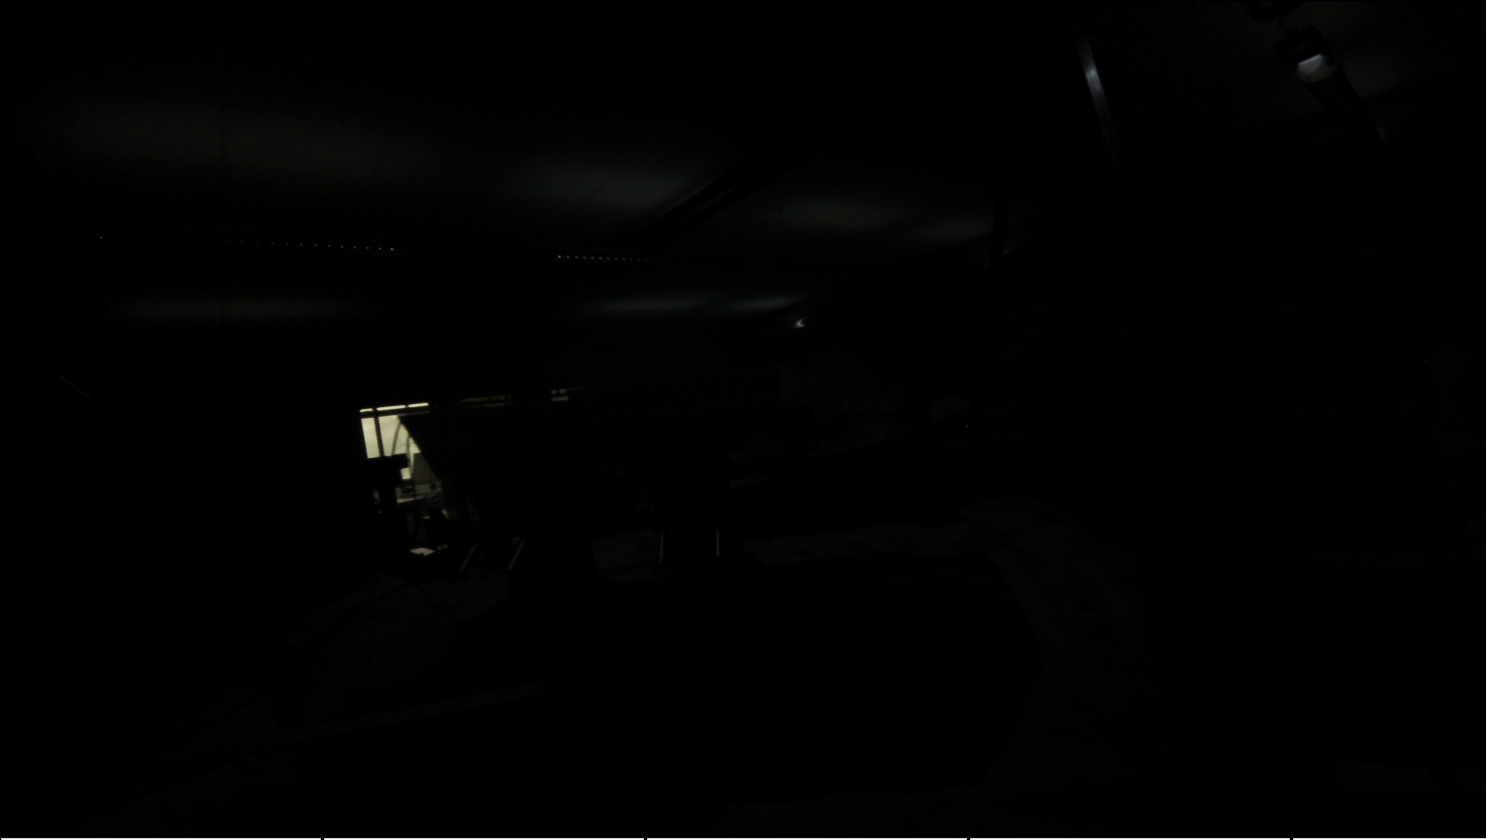
\includegraphics[width=13cm]{assets/figures/filtre_simple.png}
    \caption{Capture avec filtre - Environnement simple}
\end{figure}
\begin{figure}[H]
    \centering
    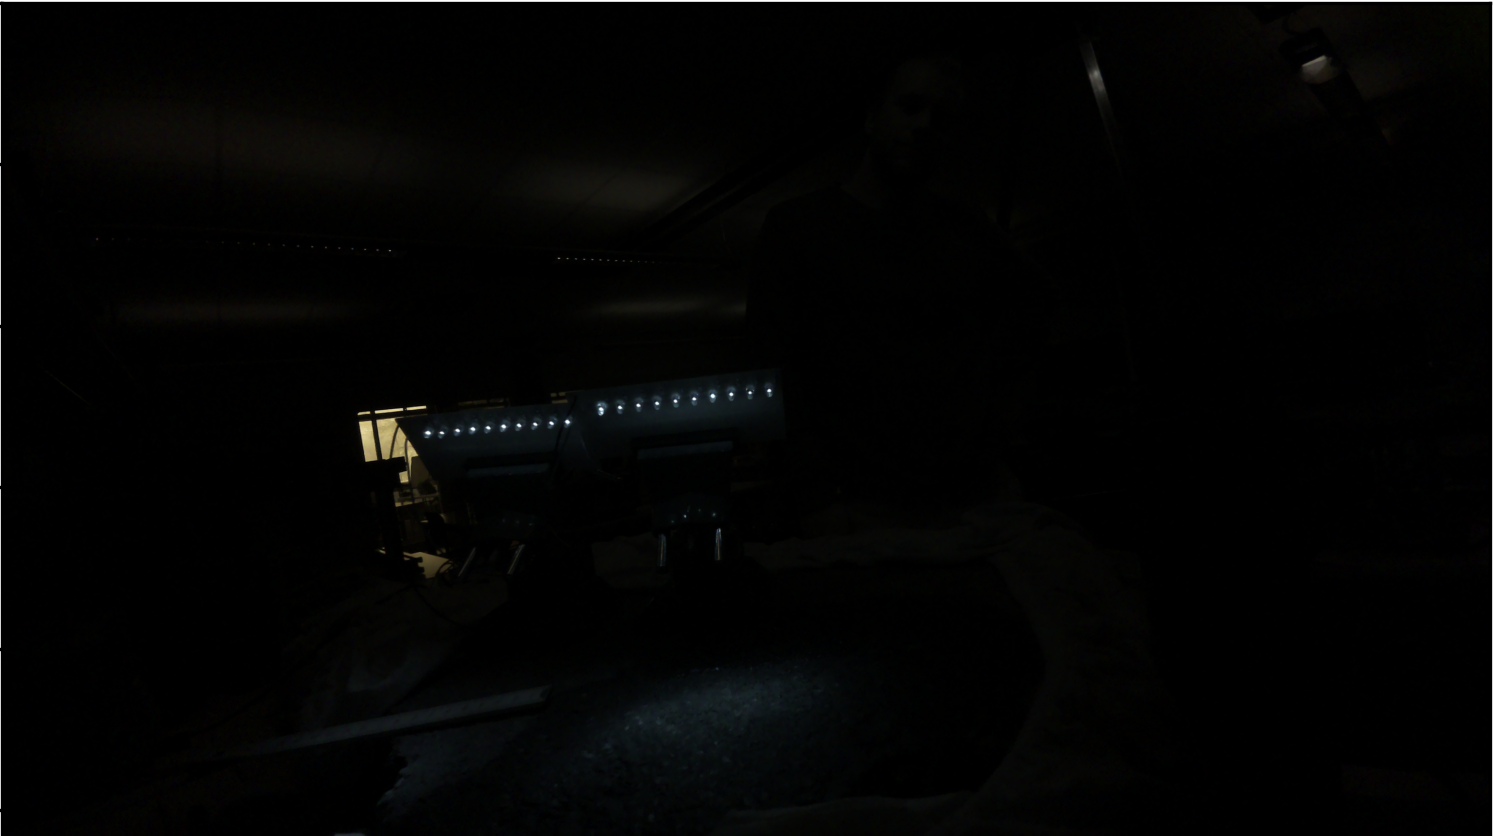
\includegraphics[width=13cm]{assets/figures/filtre_IR.png}
    \caption{Capture avec filtre - Leds IR allumées}
\end{figure}
\begin{figure}[H]
    \centering
    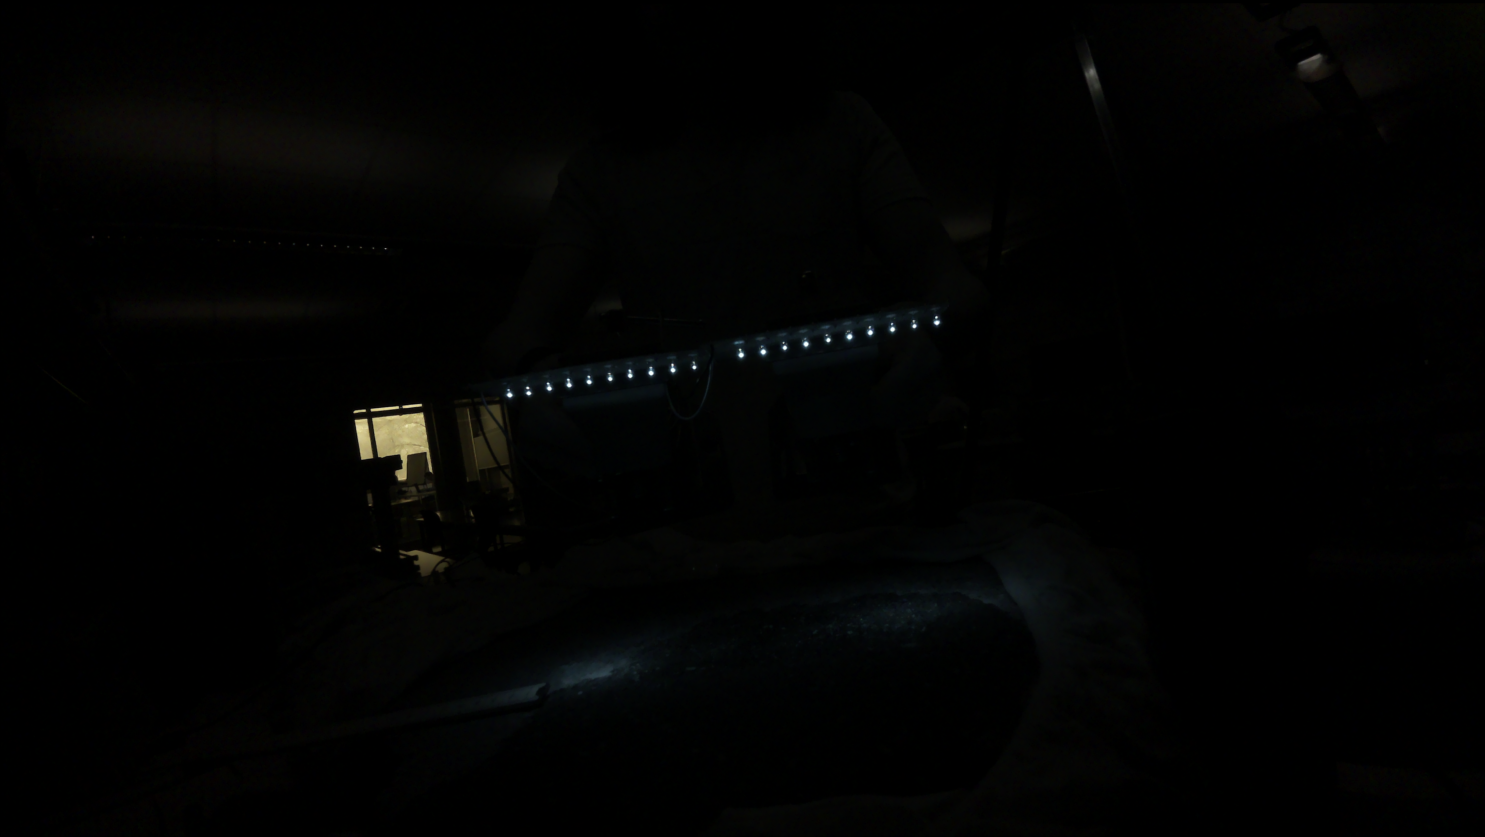
\includegraphics[width=13cm]{assets/figures/filtre_IR_huile.png}
    \caption{Capture avec filtre - Leds IR selon figure \ref{led_perp}}
\end{figure}
On observe que la quasi totalité des éclairages de la pièce disparaissent de la capture,
mettant en évidence la route et la trace d'huile au milieu de celle-ci. Il reste cependant les rayonnements solaires (visible sur la partie gauche des images)
à gérer, le soleil émettant dans un large spectre, ceux-ci apparaissent dans l'image. L'emplacement du laboratoire ne permet pas de
tester le filtre et le capteur sous un ensoleillement tel qu'on pourrait avoir en extérieur. De futurs tests sont nécessaires.

\section{Installation}
\subsection{Eclairage}
Le but est de garder le même principe d'éclairage que durant les tests préliminaires, c'est à dire une éclairage perpendiculaire au sol,
en bande, avec des leds IR émettant à 850nm. De plus, il faudrait que le système d'éclairage suive les contraintes suivantes:
\begin{itemize}
    \item Diffusion en bande.
    \item Largeur de 150cm.
    \item Repliable si non utilisés.
    \item Protégé pendant les déplacements.
\end{itemize}
J'envisage de faire fabriquer le rails de leds sur les principes suivants:
\begin{enumerate}
    \item Element solide sur lequel braser les leds (veroboard).
    \item Structure solide sur lequel fixer les veroboards (rail).
    \item Element de fixation permettant un repliage.
    \item Tube de protection à enfiler lors des transports.
\end{enumerate}
\subsubsection{Veroboard}
+ plan d'implantation

+ image résultat
\subsubsection{Rails}
\subsubsection{Fixation}
\subsubsection{Protection}
\subsection{Caméra}

\section{Programme}
\subsection{Traitement de l'image}
\subsection{Communication}
